\documentclass[fleqn]{article}
\usepackage{NotesTeX}

\usepackage{charter}

\usepackage{amsmath,amssymb}
\usepackage{enumitem}
\usepackage{tcolorbox}
\usepackage{tikz-cd}
\usepackage{amscd}
\usepackage{mathtools}
\usepackage{dsfont}
\usepackage{colortbl}
\usepackage{booktabs}
\usepackage{multirow}
\usepackage{longtable}
\usepackage{float}
\usepackage{comment}

\usepackage{pgfplots}
\pgfplotsset{compat=1.17}
\usepackage{tikz-3dplot-circleofsphere}

\providecommand{\tightlist}{%
  \setlength{\itemsep}{0pt}\setlength{\parskip}{0pt}}

\renewcommand{\leq}{\leqslant}
\renewcommand{\geq}{\geqslant}

\definecolor{primary}{RGB}{177,98,78}
\definecolor{secondary}{RGB}{91,132,177}

\usepackage{hyperref}
\hypersetup{linkcolor={secondary},urlcolor={primary}}
\usepackage[noabbrev,capitalise,nameinlink]{cleveref}
\crefformat{equation}{(#2#1#3)}


\newenvironment{idea}{\noindent}{\medskip}

\tcolorboxenvironment{idea}{
  boxrule=2pt,
  boxsep=3pt,
  colback={white},
  colframe={secondary},
  enhanced jigsaw,
  rounded corners,
  before skip=10pt,
  after skip=10pt,
}

\newenvironment{technical}{\noindent}{\medskip}

\tcolorboxenvironment{technical}{
  boxrule=2pt,
  boxsep=3pt,
  colback={white},
  colframe={primary},
  enhanced jigsaw,
  rounded corners,
  before skip=10pt,
  after skip=10pt,
}

\newtheorem*{scenario}{Scenario}

\tcolorboxenvironment{scenario}{
  boxrule=2pt,
  boxsep=3pt,
  colback={white},
  colframe={gray},
  enhanced jigsaw,
  rounded corners,
  before skip=10pt,
  after skip=10pt,
}

\newtheorem*{circuit}{Circuit}

\tcolorboxenvironment{circuit}{
  boxrule=2pt,
  boxsep=3pt,
  colback={white},
  colframe={gray},
  enhanced jigsaw,
  rounded corners,
  before skip=10pt,
  after skip=10pt,
}


\renewcommand{\footnote}[1]{\en{#1}}

\let\oldsection\section
\renewcommand\section{\clearpage\oldsection}
\let\oldpart\part
\renewcommand\part{\clearpage\oldpart}


\pagestyle{fancy}
\lhead{\thesubsection\,\,{\itshape\rightmark}}
\rhead{\thepage}
\fancyfoot{}


\usepackage{etoolbox}
\AtBeginEnvironment{quote}{\itshape}



\title{Noções básicas de computação quântica}
\author{\href{http://lattes.cnpq.br/3242250540541623}{Adriano B. Barreto}}
\date{Última atualização: 23 de outubro de 2022 \href{https://github.com/abbarreto/book-MQ}{(histórico de mudanças)}}


\usepackage{amsthm}
\newtheorem{theorem}{Theorem}[chapter]
\newtheorem{lemma}{Lemma}[chapter]
\newtheorem{corollary}{Corollary}[chapter]
\newtheorem{proposition}{Proposition}[chapter]
\newtheorem{conjecture}{Conjecture}[chapter]
\theoremstyle{definition}
\newtheorem{definition}{Definition}[chapter]
\theoremstyle{definition}
\newtheorem{example}{Example}[chapter]
\theoremstyle{definition}
\newtheorem{exercise}{Exercise}[chapter]
\theoremstyle{definition}
\newtheorem{hypothesis}{Hypothesis}[chapter]
\theoremstyle{remark}
\newtheorem*{remark}{Remark}
\newtheorem*{solution}{Solution}
\begin{document}


\setcounter{tocdepth}{2}
\maketitle

\hypertarget{prefuxe1cio}{%
\chapter*{Prefácio}\label{prefuxe1cio}}
\addcontentsline{toc}{chapter}{Prefácio}

\providecommand{\xmapsto}[1]{\overset{#1}{\longmapsto}}
\providecommand{\bra}[1]{\langle#1|}
\providecommand{\ket}[1]{|#1\rangle}
\providecommand{\braket}[2]{\langle#1|#2\rangle}
\providecommand{\proj}[1]{|#1\rangle\langle#1|}
\providecommand{\av}[1]{\langle#1\rangle}
\providecommand{\tr}{\operatorname{tr}}
\providecommand{\id}{\mathbf{1}}
\providecommand{\diag}[2]{\begin{bmatrix}#1&0\\0&#2\end{bmatrix}}
\providecommand{\mqty}[1]{\begin{matrix}#1\end{matrix}}
\providecommand{\bmqty}[1]{\begin{bmatrix}#1\end{bmatrix}}
\renewcommand{\leq}{\leqslant}
\renewcommand{\geq}{\geqslant}
\newcommand{\coloneqq}{\mathrel{=}}

For the past however-many years, \href{https://www.arturekert.com/}{Artur Ekert} has been teaching the masters course ``Introduction to Quantum Information'' at the University of Oxford.
During this time, many versions of accompanying lecture notes have come and gone, with constant improvements and changes being made.
The version that you will find on this website was originally edited by \href{https://thosgood.com}{Tim Hosgood} into a cohesive ``book'', and both authors have since then added extra comments, exercises, and examples.

\begin{quote}
\emph{Although almost complete, this book is still a work-in-progress --- a few sections are missing, but we are constantly updating and filling in the gaps!}
\emph{Note that, because of this, external links to specific chapters or sections might break as things move around.}
\end{quote}

\hypertarget{objetivos-e-puxfablico-alvo}{%
\section*{Objetivos e público-alvo}\label{objetivos-e-puxfablico-alvo}}
\addcontentsline{toc}{section}{Objetivos e público-alvo}

In this series of lectures you will learn how inherently quantum phenomena, such as quantum interference and quantum entanglement, can make information processing more efficient and more secure, even in the presence of noise.

There are many introductions to quantum information science, so it seems like a good idea to start with an explanation of why this particular one exists.
When learning such a subject, located somewhere in between mathematics, physics, and computer science, there are many possible approaches, with one main factor being ``how far along the informal--formal scale do I want to be?''.
In these notes we take the following philosophy: it can be both interesting and fun to cover lots of ground quickly and see as much as possible on a surface level, but it's also good to know that there is a lot of important stuff that you'll miss by doing this.
In practice, this means that we don't worry to much about high-level mathematics.
That is not to say that we do not use mathematics ``properly'' --- you'll find a perfectly formal treatment of e.g.~quantum channels via completely positive trace-preserving maps in the language of linear algebra --- but rather than putting too many footnotes with technical caveats and explanations throughout the main text, we opt to collect them all together into one big ``warning'' here:

\begin{quote}
\emph{The mathematics underlying quantum theory is a vast and in-depth subject, most of which we will never touch upon, some of which we will only allude to, and the rest of which we will cover only in the level of detail necessary to our overarching goal}.\footnote{However, since mathematicians were involved in the writing of this book, we have not been able to resist \emph{some} digressions here and there.}
``What'', then, ``is the overarching goal?'' one might ask.
Our answer is this:
\end{quote}

\begin{quote}
\emph{To help an eager reader understand what quantum information science is all about, and for them to realise which facets of it they would like to study in more detail}.
But this does not mean that our treatment is cursory!
In fact, by the end of this book you will have learnt a fair bit more than what might usually be covered in a standard quantum information science course that you would find in a mathematics masters degree, for example.
\end{quote}

The interdisciplinary nature of this topic, combined with the diverse backgrounds that different readers have, means that some may find certain chapters easy, while others find the same ones difficult --- so if things seem hard to you, then don't worry: the next chapter might feel much easier!
The only real prerequisites are a working knowledge of complex numbers and vectors and matrices; some previous exposure to elementary probability theory and Dirac bra-ket notation (for example) would be helpful, but we provide crash-course introductions to some topics like these at the end of this chapter.
A basic knowledge of quantum mechanics (especially in the simple context of finite dimensional state spaces, e.g.~state vectors, composite systems, unitary matrices, Born rule for quantum measurements) and some ideas from classical theoretical computer science (complexity theory, algorithms) would be helpful, but is \emph{not at all} essential.

Of course, even if you aren't familiar with the formal mathematics, then that shouldn't stop you from reading this book if you want to.
You might be surprised at how much you can \href{https://en.wikipedia.org/wiki/Black_box}{black box} the bits that you don't understand!
The caveat stands, however, that, to \emph{really} get to grips with this subject, at least some knowledge of maths is necessary --- but this is not a bad thing!

Finally, throughout this text you will find some technical asides (marked with the icon).
These are \emph{not at all} necessary reading, but are just there to provide the exceptionally eager reader (or perhaps those with a more formal mathematical background) with some extra context, as well as some pointers towards further reading.

\hypertarget{usando-este-e-book}{%
\section*{Usando este e-book}\label{usando-este-e-book}}
\addcontentsline{toc}{section}{Usando este e-book}

This book has some functionality unique to the online (as opposed to the PDF) version, accessed using the toolbar along the top of the window.
From left to right, the icons have the following use:

\begin{itemize}
\tightlist
\item
  --- Hide/show the table of contents
\item
  --- Search within the text of the book
\item
  --- Change font size, font face, and toggle dark mode
\item
  --- View the source file of the current chapter on GitHub\footnote{The GitHub-savvy of you can use this to create issues pointing out typos, mistakes, etc.}
\item
  --- Open the PDF version of the book in a new tab
\end{itemize}

The online version also has \href{https://www.youtube.com/playlist?list=PLkespgaZN4gmu0nWNmfMflVRqw0VPkCGH}{the accompanying lecture videos} embedded from YouTube.
These videos are hidden by default, but can be shown by clicking on the title next to the icon, wherever one appears.
The order of the videos generally differs from that of the written notes, so we have made our best efforts to include them in an order which makes sense relative to the chapters here.
For those wishing to really get familiar with this subject, we recommend separately watching the lecture videos following the order in \href{https://www.youtube.com/playlist?list=PLkespgaZN4gmu0nWNmfMflVRqw0VPkCGH}{the linked playlist}.

You will also see the icon in certain places.
Clicking on these will display one of the technical asides mentioned in the introduction.

If a hyperlink has the icon after it, then it points to a webpage \emph{outside} this book; otherwise it is an \emph{internal} link to another section within this book.

There are also some keyboard shortcuts:

\begin{itemize}
\tightlist
\item
  jump between sections with \texttt{←} and \texttt{→}
\item
  toggle the table of contents with \texttt{s}
\item
  open the search bar with \texttt{f}, step through results with \texttt{Enter}, and stop searching with \texttt{Esc}
\end{itemize}

\hypertarget{agradecimentos}{%
\section*{Agradecimentos}\label{agradecimentos}}
\addcontentsline{toc}{section}{Agradecimentos}

We thank the following for their helpful comments and corrections: Zhenyu Cai, Jedrzej Burkat, Maryam Khaqan.
We also appreciate the work of Yihui Xie in developing the \href{https://bookdown.org/yihui/bookdown/}{Bookdown package} with which this e-book was built.

\hypertarget{part-tuxf3picos-introdutuxf3rios}{%
\part{Tópicos Introdutórios}\label{part-tuxf3picos-introdutuxf3rios}}

\hypertarget{preliminares-matematicas}{%
\chapter{Preliminares matemáticas}\label{preliminares-matematicas}}

Here we quickly recall most of the fundamental mathematical results that we will rely on in the rest of this book, most importantly \emph{linear algebra over the complex numbers}.
However, we will not introduce everything from the ground up.
Most notably, we will assume that the reader understands what a \textbf{matrix} is, and how it represents a \textbf{linear transformation}; some prior exposure to \textbf{complex numbers} would be helpful.

If an equation like \(\operatorname{tr}|a\rangle\langle b|=\langle b|a\rangle\) makes sense to you, then you can safely skip over this section and get started directly with Chapter \ref{quantum-interference}.

As a small note on notation, we generally write ``\(x\mathrel{=}y\)'' to mean ``\(x\) is defined to be (equal to) \(y\)'', and ``\(x\equiv y\)'' to mean ``\(x\) is just another name for \(y\)'', but sometimes we simply just write ``\(x=y\)''.

\hypertarget{complex-numbers}{%
\section{Complex numbers}\label{complex-numbers}}

One of the fundamental ingredients of quantum information science (and, indeed, of quantum physics in general) is the notion of \textbf{complex numbers}.
It would be disingenuous to expect that a few paragraphs would suffice to make the reader sufficiently familiar with subject, but we try our best here to give a speedy overview of the core principles, and end with some exercises that can be a helpful indicator as to what things you might want to read up on elsewhere.

The ``classical'' way of arriving at complex numbers is as follows: start with the \textbf{natural numbers} \(\mathbb{N}=\{0,1,2,\ldots\}\), which we can add; if we want to be able to invert addition (i.e.~subtract), then we end up with the \textbf{integers} \(\mathbb{Z}=\{\ldots,-2,-1,0,1,2,\ldots\}\), which we can multiply; if we want to be able to invert multiplication (i.e.~divide), then we end up with the \textbf{rationals} \(\mathbb{Q}=\{\frac{p}{q}\mid p,q\in\mathbb{Z}\}\).
In this process of ``closure under more and more binary operations'', we have passed from a \textbf{monoid}, to a \textbf{group}, to a \textbf{field}.
Algebraically, then, we seem to be done: we can do all the addition and multiplication that we like, and we can invert it whenever it makes sense to do so (e.g.~we can divide, as long as it's not by \(0\)).

But there are lots of numbers that turn up in geometry that are not rational, such as \(\sqrt{2}\approx1.414\), \(\pi\approx3.14\), and \(e\approx2.718\).
To include all of these (and simultaneously make sense of things like infinite sums, and limits), we must do some \textbf{real analysis} --- something which we won't touch upon here --- to end up with the \textbf{real numbers} \(\mathbb{R}\).
These form a field, just like the rationals, but now we don't have any ``gaps'' in our number line.
So what's left to do?

Well the reals have one big problem: they are not \textbf{algebraically closed}.
That is, there exist polynomials with no roots, i.e.~equations of the form \(a_nx^n+a_{n-1}x^{n-1}+\ldots+a_1x+a_0=0\) (where the \(a_i\) are real numbers) that have no solutions.\footnote{To explain why we care so much about polynomials would be the subject of a whole nother book, but one important reason (of the \emph{many}!), for both analysts and geometers alike, is the \href{https://en.wikipedia.org/wiki/Stone\%E2\%80\%93Weierstrass_theorem}{\textbf{Weierstrass Approximation Theorem}}.}
Somehow the most fundamental such example is the equation \(x^2+1=0\), which has no solutions, because the square of any real number must be non-negative, and so \(\sqrt{-1}\not\in\mathbb{R}\).

It turns out that if we just throw in this one extra number \(i\mathrel{=}\sqrt{-1}\) to \(\mathbb{R}\) then we can solve \emph{any} polynomial --- a theorem so important that it's known as the \textbf{fundamental theorem of algebra}.
We call the result of doing this the \textbf{complex numbers}, and denote them by \(\mathbb{C}\).

This gives us an algebraic way of understanding what a complex number is: it is a real number \(x\) plus an \textbf{imaginary} number \(iy\) (where \(y\in\mathbb{R}\))
That is, every complex number \(x+iy\) simply corresponds to a pair of real numbers \((x,y)\).
So now we can think geometrically!
We imagine the complex numbers \(\mathbb{C}\) as the 2-dimensional Euclidean space \(\mathbb{R}^2\), where the \(x\)-axis corresponds to the real part of a complex number, and the \(y\)-axis to the imaginary part.
This really is a geometric way of thinking, since now addition (and subtraction) of complex numbers (which is defined by adding their real and imaginary parts separately) is given by vector addition, as shown in Figure \ref{fig:complex-addition}.



But what about multiplication and division?
Following the rules of the game, we can figure out what the product of two complex numbers is by treating the imaginary number \(i\) as a ``formal variable'', i.e.~pretending it's just a variable in some polynomial, and then remembering that \(i=\sqrt{-1}\) at the very end:
\[
  \begin{aligned}
    (x+iy)(x'+iy')
    &= xx'+ixy'+iyx'+i^2yy'
  \\&= xx'+ixy'+iyx'-yy'
  \\&= xx'-yy'+i(xy'+yx').
  \end{aligned}
\]

Division works similarly --- the most simple example of inverting a complex number \(x+iy\) makes sense whenever \(x\) and \(y\) are both non-zero, since then we can use the trick of ``multiplying by \(1\)'':
\[
  \begin{aligned}
    \frac{1}{x+iy}
    &= \frac{1}{x+iy}\frac{x-iy}{x-iy}
  \\&= \frac{x-iy}{x^2+y^2}
  \\&= \frac{x}{x^2+y^2}-i\frac{y}{x+2+y^2}
  \end{aligned}
\]

This other complex number \(x-iy\) that we used is somehow special because it is exactly the thing we needed to make the denominator real, so we give it a name: the \textbf{complex conjugate}\footnote{The more common notation in mathematics is \(\bar{z}\) instead of \(z^\star\), but physicists tend to like the latter.} of a complex number \(z=x+iy\) is the complex number \(z^\star\mathrel{=}x-iy\).
Geometrically, this is just the reflection of the vector \((x,y)\in\mathbb{R}^2\) in the \(x\)-axis.
The product \(zz^\star=x^2+y^2\) is also important: you might recognise (from Pythagoras' theorem) that \(\sqrt{x^2+y^2}\) is exactly the length of the vector \((x,y)\), and so we call the real number \(|z|\mathrel{=}\sqrt{zz^\star}\) the \textbf{modulus} (or magnitude, norm, or absolute value).
Note then that we can simply write \(1/z=z^\star/|z|^2\).

Now things are looking somewhat nice, but the story isn't complete.
We have a good geometric intuition for what a complex number is (a vector in \(\mathbb{R}^2\)) and how to add them (vector addition), as well as what the complex conjugate and the modulus mean (reflection in the \(x\)-axis, and the length of the vector, respectively); but what about multiplication and division?

To understand these we need to switch from our \textbf{rectangular coordinates} \(z=x+iy\) to \textbf{polar coordinates} --- instead of describing a point \(z\) in \(\mathbb{R}^2\) as ``\(x\) units left/right and \(y\) units up/down'', we describe it as ``\(r\) units from the origin, at an angle of \(\theta\) \href{https://en.wikipedia.org/wiki/Radian}{\textbf{radians}}''.
We already know, given \((x,y)\in\mathbb{R}^2\), how to calculate its distance \(r\) from the origin, since this is exactly the length of the vector: \(r=|(x,y)|=\sqrt{x^2+y^2}\).
But what about the angle?
Some trigonometry tells us that \(\theta=\tan(y/x)\), so we now know how to convert rectangular to polar coordinates:
\[
  x+iy = (x,y)
  \longmapsto (r,\theta) \mathrel{=}(\sqrt{x^2+y^2},\tan(y/x)).
\]

It would be nice to know how to go in the other direction though, but this can also be solved with some trigonometry:
\[
  (r,\theta)
  \longmapsto (r\cos\theta,r\sin\theta).
\]



Great!
\ldots{} but what's the point of polar coordinates?
Well, it turns out that they give us a geometric way of understanding multiplication: you can show\footnote{\textbf{Exercise.} Prove this!} that \((r,\theta)\) multiplied by \((r',\theta')\) is exactly \((rr',\theta+\theta')\), which says that multiplication by a complex number \((r,\theta)\) is exactly a scaling by a factor of \(r\) and a rotation by \(\theta\).
This means that we can also easily find the multiplicative inverse of \((r,\theta)\), since it's just \((1/r,-\theta)\).
Finally, complex conjugation just means switching the sign of the angle: \((r,\theta)^\star=(r,-\theta)\).

There is one last ingredient that we should mention, which is the thing that really solidifies the relation between rectangular and polar coordinates.
We know that rectangular coordinates \((x,y)\) can be written as \(x+iy\), so is there some more algebraic way of writing polar coordinates \((r,\theta)\)?
Then we can avoid any ambiguity that might arise from using pairs of numbers --- if I tell you that I'm thinking of the complex number \(z=(0.3,2)\), do I mean the point \(0.3+2i\), or the point that is distance \(r\) from the origin at an angle of \(2\) radians?

Given polar coordinates \((r,\theta)\), we know that this is equal to \((r\cos\theta,r\sin\theta)\) in rectangular coordinates.
For simplicity, let's first consider the case where \(r=1\).
Then we can write \((1,\theta)\) as \(\cos\theta+i\sin\theta\).
Using the \href{https://en.wikipedia.org/wiki/Taylor_series}{\textbf{Taylor series}}\footnote{If you don't know about Taylor series, then feel free to just skim this part, but make sure to read the punchline!} of \(\sin\) and \(\cos\), we can rewrite this as
\[
  \begin{aligned}
    \cos\theta+i\sin\theta
    &= \left(
      1-\frac{\theta^2}{2!}+\frac{\theta^4}{4!}-\ldots
    \right) + i\left(
      \theta-\frac{\theta^3}{3!}+\frac{\theta^5}{5!}-\ldots
    \right)
  \\&= 1+i\theta-\frac{\theta^2}{2!}-i\frac{\theta^3}{3!}+\frac{\theta^4}{4!}+i\frac{\theta^5}{5!}-\ldots
  \\&= 1+i\theta+\frac{i^2\theta^2}{2!}+\frac{i^3\theta^3}{3!}+\frac{i^4\theta^4}{4!}+\frac{i^5\theta^5}{5!}+\ldots
  \\&= \exp(i\theta)
  \end{aligned}
\]
where at the very end we use the Taylor expansion of the \href{https://en.wikipedia.org/wiki/Exponential_function}{\textbf{exponential function}} \(\exp(x)=e^x\).

We have just ``proved''\footnote{It is very important to point out that this ``proof'' is not rigorous or formal --- you need to be very \emph{very} careful when rearranging infinite sums! However, this proof \emph{can be made rigorous} by using some real analysis.} one of the most remarkable formulas in mathematics: \textbf{Euler's formula}
\[
  e^{i\theta} = \cos\theta+i\sin\theta
\]
(a special case of which gives the famous equation \(e^{i\pi}+1=0\), uniting five fundamental constants: \(0\), \(1\), \(i\), \(e\), and \(\pi\)).
In summary then, we have two beautiful ways of expressing a complex number \(z\in\mathbb{C}\), in either its rectangular/planar form or its polar/Euler form:
\[
  z = x+iy = re^{i\theta}.
\]

\begin{idea}
Addition and subtraction are most neatly expressed in the planar form \(x+iy\), and multiplication and division are most neatly expressed in the polar form \(re^{i\theta}\); complex conjugation looks nice and tidy in both.

\end{idea}

\begin{technical}
We know how to perform addition, multiplication, inversion (which is a special case of division), and complex conjugation on complex numbers in planar form, but we've only described how to do the last \emph{three} of these in polar form: we haven't said how to write \(re^{i\theta}+r'e^{i\theta'}\) as \(se^{i\varphi}\) for some \(s\) and \(\varphi\).
This is because it is very messy looking:
\[
  \begin{aligned}
    s
    &= \sqrt{r^2+(r')^2+2rr'\cos(\theta'-\theta)}
  \\\varphi
    &= \theta+\operatorname{atan2}\big(r'\sin(\theta'-\theta),r+r'\cos(\theta'-\theta)\big)
  \end{aligned}
\]
and where \(\operatorname{atan2}\) is the \href{https://en.wikipedia.org/wiki/Atan2}{2-argument arctangent function}.

\end{technical}

You do not need to know everything about this whole story of algebraically closed fields and so on, but it helps to know the basics, so here are some exercises that should help you to become more familiar.\footnote{Note that we have not really given you enough information in this section to be able to solve all these exercises, but that is intentional! Sometimes we like to ask questions and not answer them, with the hope that you will enjoy getting to do some research by yourself.}

\begin{enumerate}
\def\labelenumi{\alph{enumi}.}
\tightlist
\item
  The set \(\mathbb{Q}\) of rational numbers and the set \(\mathbb{R}\) of real numbers are both fields, but the set \(\mathbb{Z}\) of integers is not. Why not?
\item
  Look up the formal statement of the fundamental theorem of algebra.
\item
  Evaluate each of the following quantities:
  \[
   1+e^{-i\pi},
   \quad
   |1+i|,
   \quad
   (1+i)^{42},
   \quad
   \sqrt{i},
   \quad
   2^i,
   \quad
   i^i.
    \]
\item
  Here is a simple ``proof'' that \(+1=-1\):
  \[
   1=\sqrt{1}=\sqrt{(-1)(-1)}=\sqrt{-1}\sqrt{-1}=i^2=-1.
    \]
  What is wrong with it?
\item
  Prove that, for any two complex numbers \(w,z\in\mathbb{C}\), we always have the inequality
  \[
   |z-w| \geqslant|z|-|w|.
    \]
  \emph{Hint: use polar form, draw a diagram, and appeal to the \href{https://en.wikipedia.org/wiki/Triangle_inequality}{\textbf{triangle inequality}}!}
\item
  Using the fact that \(e^{3i\theta}=(e^{i\theta})^3\), derive a formula for \(\cos3\theta\) in terms of \(\cos\theta\) and \(\sin\theta\).
\end{enumerate}

\hypertarget{euclidean-vectors-and-vector-spaces}{%
\section{Euclidean vectors and vector spaces}\label{euclidean-vectors-and-vector-spaces}}

We assume that you are familiar with Euclidean vectors --- those arrow-like geometric objects which are used to represent physical quantities, such as trajectories, velocities, or forces.
You know that any two velocities can be added to yield a third, and the multiplication of a ``velocity vector'' by a real number is another ``velocity vector''.
So a \textbf{linear combination} of vectors is another vector: if \(v\) and \(w\) are vectors, and \(\lambda\) and \(\mu\) are numbers (rational, real, or complex, for example), then \(\lambda v+\mu w\) is another vector.
Mathematicians have simply taken these properties and defined vectors as \emph{anything} that we can add and multiply by numbers, as long as everything behaves in a nice enough way.
This is basically what an Italian mathematician Giuseppe Peano (1858--1932) did in a chapter of his 1888 book with an impressive title: \emph{Calcolo geometrico secondo l'Ausdehnungslehre di H. Grassmann preceduto dalle operazioni della logica deduttiva}.
Following Peano, we define a \textbf{vector space} as a mathematical structure in which the notion of linear combination ``makes sense''.

More formally, a \textbf{complex vector space} is a set \(V\) such that, given any two \textbf{vectors} \(a\) and \(b\) (that is, any two elements of \(V\)) and any two \emph{complex} numbers \(\alpha\) and \(\beta\), we can form the linear combination \(\alpha a+\beta b\), which is also a vector in \(V\).
There are certain ``nice properties'' that vector spaces things must satisfy. Addition of vectors must be commutative and associative, with an identity (the zero vector, which is often written as \(\mathbf{0}\)) and an inverse for each \(v\) (written as \(-v\)). Multiplication by complex numbers must obey the two distributive laws: \((\alpha+\beta)v = \alpha v+\beta v\) and \(\alpha (v+w) = \alpha v+\alpha w\).

\begin{technical}
A more succinct way of defining a vector space is as an abelian group endowed with a scalar action of a field.
This showcases vector spaces as a particularly well behaved example of a more general object: \textbf{modules over a ring}.

\end{technical}

A \textbf{subspace} of \(V\) is any subset of \(V\) which is closed under vector addition and multiplication by complex numbers.
Here we start using the Dirac bra-ket notation and write vectors in a somewhat fancy way as \(|\text{label}\rangle\), where the ``label'' is anything that serves to specify what the vector is.
For example, \(|\uparrow\rangle\) and \(|\downarrow\rangle\) may refer to an electron with spin up or down along some prescribed direction, and \(|0\rangle\) and \(|1\rangle\) may describe a quantum bit holding either logical \(0\) or \(1\).
As a maybe more familiar example, the set of binary strings of length \(n\) is a vector space over the field \(\mathbb{Z}/2\mathbb{Z}\) of integers mod \(2\); in the case \(n=2\) we can write down all the vectors in this vector space in this notation: \(|00\rangle\), \(|01\rangle\), \(|10\rangle\), \(|11\rangle\), where e.g.~\(|10\rangle+|11\rangle=|01\rangle\) (addition is taken mod \(2\)).
These are often called \textbf{ket} vectors, or simply \textbf{kets}.
(We will deal with ``bras'' in a moment).

A \textbf{basis} in \(V\) is a collection of vectors \(|e_1\rangle,|e_2\rangle,\ldots,|e_n\rangle\) such that every vector \(|v\rangle\) in \(V\) can be written (in \emph{exactly} one way) as a linear combination of the basis vectors: \(|v\rangle=\sum_{i=1}^n v_i|e_i\rangle\).
The number of elements in a basis is called the \textbf{dimension} of \(V\).\footnote{Showing that this definition is independent of the basis that we choose is a ``fun'' linear algebra exercise.}
The most common, and prototypical, \(n\)-dimensional complex vector space (and the space which we will be using most of the time) is the space of ordered \(n\)-tuples of complex numbers, usually written as column vectors:
\[
  |a\rangle
  = \begin{bmatrix}a_1\\a_2\\\vdots\\a_n\end{bmatrix}
\]
with a basis given by the column vectors \(|e_i\rangle\) that are \(0\) in every row except for a \(1\) in the \(i\)-th row:
\[
  |e_1\rangle
  = \begin{bmatrix}1\\0\\\vdots\\0\end{bmatrix}
  \qquad
  |e_2\rangle
  = \begin{bmatrix}0\\1\\\vdots\\0\end{bmatrix}
  \qquad\ldots\qquad
  |e_n\rangle
  = \begin{bmatrix}0\\0\\\vdots\\1\end{bmatrix}
\]
and where addition of vectors is done \textbf{component-wise}, so that
\[
  \left(\sum_{i=1}^n v_i|e_i\rangle\right)+\left(\sum_{i=1}^n w_i|e_i\rangle\right)
  = \sum_{i=1}^n (v_i+w_i)|e_i\rangle
\]
or, in column vectors,
\[
  \begin{gathered}
    |v\rangle
    = \begin{bmatrix}v_1\\v_2\\\vdots\\v_n\end{bmatrix}
    \qquad
    |w\rangle
    = \begin{bmatrix}w_1\\w_2\\\vdots\\w_n\end{bmatrix}
  \\\alpha|a\rangle+\beta|b\rangle
    = \begin{bmatrix}\alpha v_1+\beta w_1\\\alpha v_2+\beta w_2\\\vdots\\\alpha v_n+\beta w_n\end{bmatrix}
  \end{gathered}
\]

Throughout the course we will deal only with vector spaces of \emph{finite} dimensions.
This is sufficient for all our purposes and we will avoid many mathematical subtleties associated with infinite dimensional spaces, for which we would need the tools of \textbf{functional analysis}.

Formally, whenever we say \textbf{\(n\)-dimensional Euclidean space}, we mean the \emph{real} vector space \(\mathbb{R}^n\).

\hypertarget{bras-and-kets}{%
\section{Bras and kets}\label{bras-and-kets}}

An \textbf{inner product} on a vector space \(V\) (over the complex numbers) is a function that assigns to each pair of vectors \(|u\rangle,|v\rangle\in V\) a complex number \(\langle u|v\rangle\), and satisfies the following conditions:

\begin{itemize}
\tightlist
\item
  \(\langle u|v\rangle=\langle v|u\rangle^\star\)
\item
  \(\langle v|v\rangle\geqslant 0\) for all \(|v\rangle\)
\item
  \(\langle v|v\rangle= 0\) if and only if \(|v\rangle=0\)
\end{itemize}

where \({}^\star\) denotes complex conjugation (sometimes written as \(z\mapsto\bar{z}\) instead).

The inner product must also be \emph{linear} in the second argument but \emph{antilinear} in the first argument:
\[
  \langle c_1u_1+c_2u_2|v\rangle = c_1^\star\langle u_1|v\rangle+c_2^\star\langle u_2|v\rangle
\]
for any complex constants \(c_1\) and \(c_2\).

To any physical system we associate\footnote{The question of \emph{how} exactly we construct this associated space is a subtle one in the case of arbitrary physical systems, but we shall see that this is relatively straightforward when working with the types of systems that we consider in this book.} a complex vector space with an inner product, known as a \textbf{Hilbert space} \(\mathcal{H}\).
The inner product between vectors \(|u\rangle\) and \(|v\rangle\) in \({\mathcal{H}}\) is written as \(\langle u|v\rangle\).

\begin{technical}
If \(V\) is a vector space with an inner product \(\langle-,-\rangle\), then this gives us a \textbf{norm} on \(V\) by defining \(\|x\|=\sqrt{\langle x,x\rangle}\) and thus a \textbf{metric} by defining \(d(x,y)=\|y-x\|\).
We say that a sequence \((x_n)\) in \(V\) is \textbf{Cauchy} if its elements ``eventually always get closer'', i.e.~if for all \(\varepsilon>0\) there exists some \(N\in\mathbb{N}\) such that for all \(m,n>N\) we have \(\|x_n-x_m\|<\varepsilon\).
We say that a normed space is \textbf{complete} if \emph{every Cauchy sequence converges in that space}, i.e.~if the limits of sequences that \emph{should} exist actually \emph{do} exist.

Now one useful fact is the following: on a \emph{finite dimensional} vector space, all norms are equivalent.
(Note that this does \emph{not} mean that \(\|x\|_1=\|x\|_2\) for any two norms \(\|-\|_1\) and \(\|-\|_2\), but simply that they ``induce the same topology'' --- feel free to look up the precise definition elsewhere).
This follows from another useful fact: in a \emph{finite dimensional} vector space, the unit ball is compact.
By a short topological argument, we can use these facts to show that what we claimed, namely that every \emph{finite dimensional} inner product space is complete (with respect to the norm induced by the inner product, and thus with respect to \emph{any} norm, since all norms are equivalent).

In the infinite dimensional case these facts are \emph{not} true, and we have a special name for those inner product spaces which \emph{are} complete: \textbf{Hilbert spaces}.
So working in the finite dimensional case means that ``we do not have to worry about analysis'', in that the completeness property comes for free the moment we have an inner product, and we can freely refer to inner product spaces as Hilbert spaces.

\end{technical}

For example, for column vectors \(|u\rangle\) and \(|v\rangle\) in \(\mathbb{C}^n\) written as
\[
  |u\rangle
  = \begin{bmatrix}u_1\\u_2\\\vdots\\u_n\end{bmatrix}
  \qquad
  |v\rangle
  = \begin{bmatrix}v_1\\v_2\\\vdots\\v_n\end{bmatrix}
\]
their inner product is defined by
\[
  \langle u|v\rangle
  = u_1^\star v_1 + u_2^\star v_2+\ldots + u_n^\star v_n.
\]
Following Dirac, we may split the inner product into two ingredients:
\[
  \langle u|v\rangle
  \longrightarrow \langle u|\,|v\rangle.
\]
Here \(|v\rangle\) is a ket vector, and \(\langle u|\) is called a \textbf{bra} vector, or a \textbf{bra}, and can be represented by a row vector:
\[
  \langle u|
  = \begin{bmatrix}u_1^\star,&u_2^\star,&\ldots,&u_n^\star\end{bmatrix}.
\]
The inner product can now be viewed as the result of the matrix multiplication:
\[
  \begin{aligned}
    \langle u|v\rangle
    &= \begin{bmatrix}u_1^\star,&u_2^\star,&\ldots,&u_n^\star\end{bmatrix}
    \cdot \begin{bmatrix}v_1\\v_2\\\vdots\\v_n\end{bmatrix}
  \\&= u_1^\star v_1 + u_2^\star v_2 + \ldots + u_n^\star v_n.
  \end{aligned}
\]

Bras are vectors: you can add them, and multiply them by scalars (which, here, are complex numbers), but they are vectors in the space \({\mathcal{H}}^\star\) which is \textbf{dual} to \(\mathcal{H}\).
Elements of \({\mathcal{H}}^\star\) are \textbf{linear functionals}, that is, linear maps from \(\mathcal{H}\) to \(\mathbb{C}\).
A linear functional \(\langle u|\) acting on a vector \(|v\rangle\) in \(\mathcal{H}\) gives a complex number \(\langle u|v\rangle\).

\begin{idea}
All Hilbert spaces of the same (finite) dimension are isomorphic, so the differences between quantum systems cannot be really understood without additional structure. This structure is provided by a specific algebra of operators acting on \(\mathcal{H}\).

\end{idea}

\hypertarget{daggers}{%
\section{Daggers}\label{daggers}}

Although \(\mathcal{H}\) and \(\mathcal{H}^\star\) are not identical spaces --- the former is inhabited by kets, and the latter by bras --- they are closely related.
There is a bijective map from one to the other given by \(|v\rangle\leftrightarrow \langle v|\), and denoted by a \textbf{dagger}:\footnote{``Is this a \(\dagger\) which I see before me\ldots{}''}
\[
  \begin{aligned}
    \langle v|
    &= (|v\rangle)^\dagger
  \\|v\rangle
    &= (\langle v|)^\dagger.
  \end{aligned}
\]
We usually omit the parentheses when it is obvious what the dagger operation applies to.

The dagger operation, also known as \textbf{Hermitian conjugation}, is \emph{antilinear}:
\[
  \begin{aligned}
    (c_1|v_1\rangle+c_2|v_2\rangle)^\dagger
    &= c_1^\star\langle v_1| + c_2^\star\langle v_2|
  \\(c_1\langle v_1|+c_2\langle v_2|)^\dagger
    &= c_1^\star|v_1\rangle + c_2^\star|v_2\rangle.
  \end{aligned}
\]
Also, when applied twice, the dagger operation is the identity map.

You might already be familiar with Hermitian conjugation under another name: the \textbf{conjugate transpose}\footnote{In mathematics texts this operation is often denoted by \({}^\star\) rather than \({}^\dagger\), but we reserve the former for complex conjugation \emph{without} matrix transposition. Note, however, that scalars can be thought of as \((1\times1)\) matrices, and in this special case we have that \(\dagger=\star\).} of an \((n\times m)\) matrix \(A\) is an \((m\times n)\) matrix \(A^\dagger\), obtained by interchanging the rows and columns of \(A\) and taking complex conjugates of each entry in \(A\), i.e.~\(A^\dagger_{ij}=A^\star_{ji}\).
In particular then,
\[
  |v\rangle = \begin{bmatrix}v_1\\v_2\\\vdots\\v_n\end{bmatrix}
  \overset{\dagger}{\longleftrightarrow}
  \langle v| = \begin{bmatrix}v_1^\star,&v_2^\star,&\ldots,&v_n^\star\end{bmatrix}.
\]

\hypertarget{geometry}{%
\section{Geometry}\label{geometry}}

The inner product brings geometry: the \textbf{length}, or \textbf{norm}, of \(|v\rangle\) is given by \(\|v\|=\sqrt{\langle v|v\rangle}\), and we say that \(|u\rangle\) and \(|v\rangle\) are \textbf{orthogonal} if \(\langle u|v\rangle=0\).
Any maximal set of pairwise orthogonal vectors of unit length\footnote{That is, consider sets of vectors \(|e_i\rangle\) such that \(\langle e_i|e_j\rangle=\delta_{ij}\) (where the \textbf{Kronecker delta} \(\delta_{ij}\) is \(0\) if \(i\neq j\), and \(1\) if \(i=j\).), and then pick any of the largest such sets (which must exist, since we assume our vector spaces to be finite dimensional).} forms an orthonormal basis, and so any vector can be expressed as a linear combination of the basis vectors:
\[
  \begin{gathered}
    |v\rangle
    =\sum_i v_i|e_i\rangle
  \\\text{where $v_i=\langle e_i|v\rangle$}.
  \end{gathered}
\]
Then the bras \(\langle e_i|\) form the \textbf{dual basis}
\[
  \begin{gathered}
    \langle v|
    =\sum_i v_i^\star\langle e_i|
  \\\text{where $v_i^\star=\langle v|e_i\rangle$}.
  \end{gathered}
\]

To make the notation a bit less cumbersome, we will sometimes label the basis kets as \(|i\rangle\) rather than \(|e_i\rangle\), and write
\[
  \begin{aligned}
    |v\rangle
    &= \sum_i |i\rangle\langle i|v\rangle
  \\\langle v|
    &= \sum_j \langle v|i\rangle\langle i|
  \end{aligned}
\]
but \emph{do not confuse \(|0\rangle\) with the zero vector}!
We \emph{never} write the zero vector as \(|0\rangle\), but only ever as \(0\), without any bra or ket decorations (so e.g.~\(|v\rangle+0=|v\rangle\)).

Now that we have some notion of geometry, we can explain a bit more about this idea of associating a Hilbert space to a quantum system --- we will use some terminology that we have not yet introduced, but all will be explained in due time.

\begin{idea}
To any \emph{isolated} quantum system, which can be prepared in \(n\) \textbf{perfectly distinguishable} states, we can associate a Hilbert space \(\mathcal{H}\) of dimension \(n\) such that each vector \(|v\rangle\in\mathcal{H}\) of unit length \(\langle v|v\rangle=1\) represents a quantum state of the system.
The overall phase of the vector has no physical significance: \(|v\rangle\) and \(e^{i\varphi}|v\rangle\) (for any real \(\varphi\)) both describe the same state.

\end{idea}

We note here one more fact that also won't yet make sense, but which won't hurt to have hidden away in the back of your mind.

\begin{idea}
The inner product \(\langle u|v\rangle\) is the \textbf{probability amplitude} that a quantum system prepared in state \(|v\rangle\) will be found in state \(|u\rangle\) upon measurement.
This means that states corresponding to orthogonal vectors (i.e.~\(\langle u|v\rangle=0\)) are perfectly distinguishable: if we prepare the system in state \(|v\rangle\), then it will never be found in state \(|u\rangle\), and vice versa.

\end{idea}

\hypertarget{operators}{%
\section{Operators}\label{operators}}

A \textbf{linear map} between two vector spaces \(\mathcal{H}\) and \(\mathcal{K}\) is a function \(A\colon\mathcal{H}\to\mathcal{K}\) that respects linear combinations:
\[
  A(c_1|v_1\rangle+c_2|v_2\rangle)=c_1 A|v_1\rangle+c_2 A|v_2\rangle
\]
for any vectors \(|v_1\rangle,|v_2\rangle\) and any complex numbers \(c_1,c_2\).
We will focus mostly on \textbf{endomorphisms}, that is, maps from \(\mathcal{H}\) to \(\mathcal{H}\), and we will call them \textbf{operators}.
The symbol \(\mathbf{1}\) is reserved for the identity operator that maps every element of \(\mathcal{H}\) to itself (i.e.~\(\mathbf{1}|v\rangle=|v\rangle\) for all \(|v\rangle\in\mathcal{H}\)).
The product \(BA\) of two operators \(A\) and \(B\) is the operator obtained by first applying \(A\) to some ket \(|v\rangle\) and then \(B\) to the ket which results from applying \(A\):
\[
  (BA)|v\rangle = B(A|v\rangle).
\]
The order \emph{does} matter: in general, \(BA\neq AB\).
In the exceptional case in which \(AB=BA\), one says that these two operators \textbf{commute}.
The inverse of \(A\), written as \(A^{-1}\), is the operator that satisfies \(AA^{-1}=\mathbf{1}=A^{-1}A\).
For finite-dimensional spaces, one only needs to check \emph{one} of these two conditions, since any one of the two implies the other, whereas, on an infinite-dimensional space, \emph{both} must be checked.
Finally, given a particular basis, an operator \(A\) is uniquely determined by the entries of its matrix: \(A_{ij}=\langle i|A|j\rangle\).

The \textbf{adjoint}, or \textbf{Hermitian conjugate}, of an linear map \(A\), denoted by \(A^\dagger\), is defined by the relation
\[
  \begin{gathered}
    \langle i|A^\dagger|j\rangle
    = \langle j|A|i\rangle^\star
  \\\text{for all $|i\rangle,|j\rangle\in\mathcal{H}$}
  \end{gathered}
\]
and \(\dagger\) turns \((n\times m)\) matrices into \((m\times n)\) matrices.

An operator \(A\) is said to be

\begin{itemize}
\tightlist
\item
  \textbf{normal} if \(AA^\dagger = A^\dagger A\)
\item
  \textbf{unitary} if \(A^\dagger=A^{-1}\)
\item
  \textbf{Hermitian} (or \textbf{self-adjoint}) if \(A^\dagger = A\).
\end{itemize}

In particular then, being unitary implies being normal, since if \(A^\dagger=A^{-1}\) then \(AA^\dagger=A^\dagger A\), since both of these are equal to \(\mathbf{1}\).
Note also that unitary and Hermitian operators must be operators, i.e.~they are represented by an \((n\times n)\) matrix.

Any \emph{physically admissible} evolution of an isolated quantum system is represented by a unitary operator.\footnote{This is an \emph{axiom}, justified by experimental evidence, and also by some sort of mathematical intuition. So, in this book, we take this as a \emph{fact} that we do not question. It is, however, very interesting to question it: \emph{why should we assume this to be true?}}
Note that unitary operators preserve the inner product: given a unitary operator \(U\) and two kets \(|a\rangle\) and \(|b\rangle\), and defining \(|a'\rangle=U|a\rangle\) and \(|b'\rangle=U|b\rangle\), we have that
\[
  \begin{gathered}
    \langle a'|=\langle a|U^\dagger
  \\\langle b'|=\langle b|U^\dagger
  \\\langle a'|b'\rangle=\langle a|U^\dagger U|b\rangle=\langle a|\mathbf{1}|b\rangle=\langle a|b\rangle.
  \end{gathered}
\]
Preserving the inner product implies preserving the norm induced by this product, i.e.~unit state vectors are mapped to unit state vectors, i.e.~\emph{unitary operations are the isometries of the Euclidean norm}.

\hypertarget{eigenvalues-and-eigenvectors}{%
\section{Eigenvalues and eigenvectors}\label{eigenvalues-and-eigenvectors}}

Given an operator \(A\), an \textbf{eigenvector} is a non-zero vector \(|v\rangle\) such that
\[
  A|v\rangle = \lambda|v\rangle
\]
for some \(\lambda\in\mathbb{C}\) (which is called the corresponding \textbf{eigenvalue}).
We call the pair \((\lambda,|v\rangle)\) an \textbf{eigenpair}, and we call the set of eigenvalues the \textbf{spectrum} of \(A\), denoted by \(\sigma(A)\).
It is a surprising (but incredibly useful) fact that every operator has at least one eigenpair.\footnote{You can prove this for an \((n\times n)\) matrix \(A\) by considering the set \(\{|v\rangle,A|v\rangle,A^2|v\rangle,\ldots,A^n|v\rangle\}\) of vectors in \(\mathbb{C}^n\). Since this has \(n+1\) elements, it must be linearly \emph{dependent}, and so (after some lengthy algebra) we can construct an eigenpair.}
Geometrically, an eigenvector of an operator \(A\) is a vector upon which \(A\) simply acts by ``stretching''.

Rewriting the defining property of an eigenpair \((\lambda,|v\rangle)\), we see that
\[
  (A-\lambda\mathbf{1})|v\rangle = 0
\]
which tells us that the operator \(A-\lambda\mathbf{1}\) has a non-zero kernel, and is thus non-invertible.
This gives a useful characterisation of the spectrum in terms of a determinant:
\[
  \sigma(A) = \{\lambda\in\mathbb{C} \mid \det(A-\lambda\mathbf{1})=0\}.
\]

\hypertarget{outer-products}{%
\section{Outer products}\label{outer-products}}

Apart from the inner product \(\langle u|v\rangle\), which is a complex number, we can also form the \textbf{outer product} \(|u\rangle\langle v|\), which is a linear map (operator) on \(\mathcal{H}\) (or on \(\mathcal{H}^\star\), depending how you look at it).
This is what physicists like (and what mathematicians dislike!) about Dirac notation: a certain degree of healthy ambiguity.

\begin{itemize}
\tightlist
\item
  The result of \(|u\rangle\langle v|\) acting on a ket \(|x\rangle\) is \(|u\rangle\langle v|x\rangle\), i.e.~the vector \(|u\rangle\) multiplied by the complex number \(\langle v|x\rangle\).
\item
  Similarly, the result of \(|u\rangle\langle v|\) acting on a bra \(\langle y|\) is \(\langle y|u\rangle\langle v|\), i.e.~the linear functional \(\langle v|\) multiplied by the complex number \(\langle y|u\rangle\).
\end{itemize}

The product of two maps, \(A=|a\rangle\langle b|\) followed by \(B=|c\rangle\langle d|\), is a linear map \(BA\), which can be written in Dirac notation as
\[
  BA = |c\rangle\langle d|a\rangle\langle b| = \langle d|a\rangle|c\rangle\langle b|
\]
i.e.~the inner product (complex number) \(\langle d|a\rangle\) times the outer product (linear map) \(|c\rangle\langle b|\).

Any operator on \(\mathcal{H}\) can be expressed as a sum of outer products. Given an orthonormal basis \(\{|e_i\rangle\}_{i=1,\ldots,n}\), any operator which maps the basis vectors \(|e_i\rangle\) to vectors \(|f_i\rangle\) can be written as \(\sum_{i=1}^n|f_i\rangle\langle e_i|\).
If the vectors \(\{|f_i\rangle\}\) \emph{also} form an orthonormal basis then the operator simply ``rotates'' one orthonormal basis into another.
These are unitary operators which preserve the inner product.
In particular, if each \(|e_i\rangle\) is mapped to \(|e_i\rangle\), then we obtain the identity operator:
\[
  \sum_i|e_i\rangle\langle e_i|=\mathbf{1}.
\]
This relation holds for \emph{any} orthonormal basis, and it is one of the most ubiquitous and useful formulas in quantum theory, known as \textbf{completeness}.\footnote{Not to be confused with ``completeness'' in the sense of Hilbert spaces.}
For example, for any vector \(|v\rangle\) and for any orthonormal basis \(\{|e_i\rangle\}\), we have
\[
  \begin{aligned}
    |v\rangle
    &= \mathbf{1}|v\rangle
  \\&= \sum_i |e_i\rangle\langle e_i|\;|v\rangle
  \\&= \sum_i |e_i\rangle\;\langle e_i|v\rangle
  \\&= \sum_i v_i|e_i\rangle
  \end{aligned}
\]
where \(v_i=\langle e_i|v\rangle\) are the components of \(|v\rangle\).

Finally, note that calculating the adjoint of an outer product boils down to just swapping the order:
\[
  (|a\rangle\langle b|)^\dagger = |b\rangle\langle a|.
\]

\begin{technical}
This whole package of stuff and properties and structure (i.e.~finite dimensional Hilbert spaces with linear maps and the dagger) bundles up into an abstract framework called a \href{https://en.wikipedia.org/wiki/Dagger_compact_category}{\textbf{dagger compact category}}.
We will not delve into the vast world of category theory in this book, and to reach an understanding of all the ingredients that go into the one single definition of dagger compact categories would take more than a single chapter.
But it's a good idea to be aware that there are researchers in quantum information science who work \emph{entirely} from this approach, known as \href{https://en.wikipedia.org/wiki/Categorical_quantum_mechanics}{\textbf{categorical quantum mechanics}}.

\end{technical}

\hypertarget{the-trace}{%
\section{The trace}\label{the-trace}}

The \textbf{trace} is an operation which turns outer products into inner products,
\[
  \operatorname{tr}\colon |b\rangle\langle a| \longmapsto \langle a|b\rangle.
\]
We have just seen that any linear operator can be written as a sum of outer products, and so we can extend the definition of trace (by linearity) to any operator.
Equivalently, for any square matrix \(A\), the trace of \(A\) can be defined to be the sum of its diagonal elements:
\[
  \operatorname{tr}A = \sum_k \langle e_k|A|e_k\rangle = \sum_k A_{kk}.
\]
In fact, the trace of \(A\) is equal to the sum of the eigenvalues of \(A\), even in the case where \(A\) is not diagonalisable.

You can show, using this definition or otherwise, that the trace is cyclic\footnote{Note that ``cyclic'' does not mean the same thing as ``permutation invariant''! It is \emph{not} true in general that \(\operatorname{tr}(ABC)=\operatorname{tr}(CBA)\), but only that \(\operatorname{tr}(ABC)=\operatorname{tr}(BCA)=\operatorname{tr}(CAB)\), i.e.~we can only \emph{cyclically} permute the operators.} (\(\operatorname{tr}(AB) = \operatorname{tr}(BA)\)) and linear (\(\operatorname{tr}(\alpha A+\beta B) = \alpha\operatorname{tr}(A)+\beta\operatorname{tr}(B)\), where \(A\) and \(B\) are square matrices and \(\alpha\) and \(\beta\) complex numbers).

To recover the first definition from the second, we argue as follows:
\[
  \begin{aligned}
    \operatorname{tr}|b\rangle\langle a|
    &= \sum_k \langle e_k|b\rangle\langle a|e_k\rangle
  \\&= \sum_k \langle a|e_k\rangle\langle e_k|b\rangle
  \\&= \langle a|\mathbf{1}|b\rangle
  \\&= \langle a|b\rangle.
  \end{aligned}
\]
Here, the second term can be viewed both as the sum of the diagonal elements of \(|b\rangle\langle a|\) in the \(|e_k\rangle\) basis, and as the sum of the products of two complex numbers \(\langle e_k|b\rangle\) and \(\langle a|e_k\rangle\).
We have used the decomposition of the identity, \(\sum_k|e_k\rangle\langle e_k|=\mathbf{1}\).
Given that we can decompose the identity by choosing any orthonormal basis, it is clear that the trace does \emph{not} depend on the choice of the basis.

\hypertarget{some-useful-identities}{%
\section{Some useful identities}\label{some-useful-identities}}

Here is a summary of some particularly useful equalities concerning bras, kets, inner products, outer products, traces, and operators, that we will be using time and time again.
In all of these, \(|a\rangle,|b\rangle\in\mathcal{H}\) are kets, \(A,B,C\) are operators on \(\mathcal{H}\), and \(\alpha,\beta\in\mathbb{C}\) are scalars.

Dagger for bras and kets:

\begin{itemize}
\tightlist
\item
  \(|a\rangle^\dagger = \langle a|\)
\item
  \(\langle a|^\dagger = |a\rangle\)
\item
  \((|a\rangle\langle b|)^\dagger = |b\rangle\langle a|\)
\item
  \((\alpha|a\rangle+\beta|b\rangle)^\dagger = \alpha^\star\langle a|+\beta^\star\langle b|\)
\end{itemize}

Dagger for operators:

\begin{itemize}
\tightlist
\item
  \((AB)^\dagger = B^\dagger A^\dagger\)
\item
  \((A^\dagger)^\dagger = A\)
\item
  \((\alpha A+\beta B)^\dagger = \alpha^\star A^\dagger+\beta^\star B^\dagger\)
\end{itemize}

Trace:

\begin{itemize}
\tightlist
\item
  \(\operatorname{tr}(\alpha A+\beta B) = \alpha \operatorname{tr}(A)+\beta\operatorname{tr}(B)\)
\item
  \(\operatorname{tr}(ABC) = \operatorname{tr}(CAB) = \operatorname{tr}(BCA)\)
\item
  \(\operatorname{tr}|a\rangle\langle b| = \langle b|a\rangle\)
\item
  \(\operatorname{tr}(A|a\rangle\langle b|) = \langle b|A|a\rangle = \operatorname{tr}(|a\rangle\langle b|A)\)
\end{itemize}

\hypertarget{cross}{%
\chapter{Cross-references}\label{cross}}

Cross-references make it easier for your readers to find and link to elements in your book.

\hypertarget{chapters-and-sub-chapters}{%
\section{Chapters and sub-chapters}\label{chapters-and-sub-chapters}}

There are two steps to cross-reference any heading:

\begin{enumerate}
\def\labelenumi{\arabic{enumi}.}
\tightlist
\item
  Label the heading: \texttt{\#\ Hello\ world\ \{\#nice-label\}}.

  \begin{itemize}
  \tightlist
  \item
    Leave the label off if you like the automated heading generated based on your heading title: for example, \texttt{\#\ Hello\ world} = \texttt{\#\ Hello\ world\ \{\#hello-world\}}.
  \item
    To label an un-numbered heading, use: \texttt{\#\ Hello\ world\ \{-\#nice-label\}} or \texttt{\{\#\ Hello\ world\ .unnumbered\}}.
  \end{itemize}
\item
  Next, reference the labeled heading anywhere in the text using \texttt{\textbackslash{}@ref(nice-label)}; for example, please see Chapter \ref{cross}.

  \begin{itemize}
  \tightlist
  \item
    If you prefer text as the link instead of a numbered reference use: \protect\hyperlink{cross}{any text you want can go here}.
  \end{itemize}
\end{enumerate}

\hypertarget{captioned-figures-and-tables}{%
\section{Captioned figures and tables}\label{captioned-figures-and-tables}}

Figures and tables \emph{with captions} can also be cross-referenced from elsewhere in your book using \texttt{\textbackslash{}@ref(fig:chunk-label)} and \texttt{\textbackslash{}@ref(tab:chunk-label)}, respectively.

See Figure \ref{fig:nice-fig}.

\begin{figure}[H]

{\centering 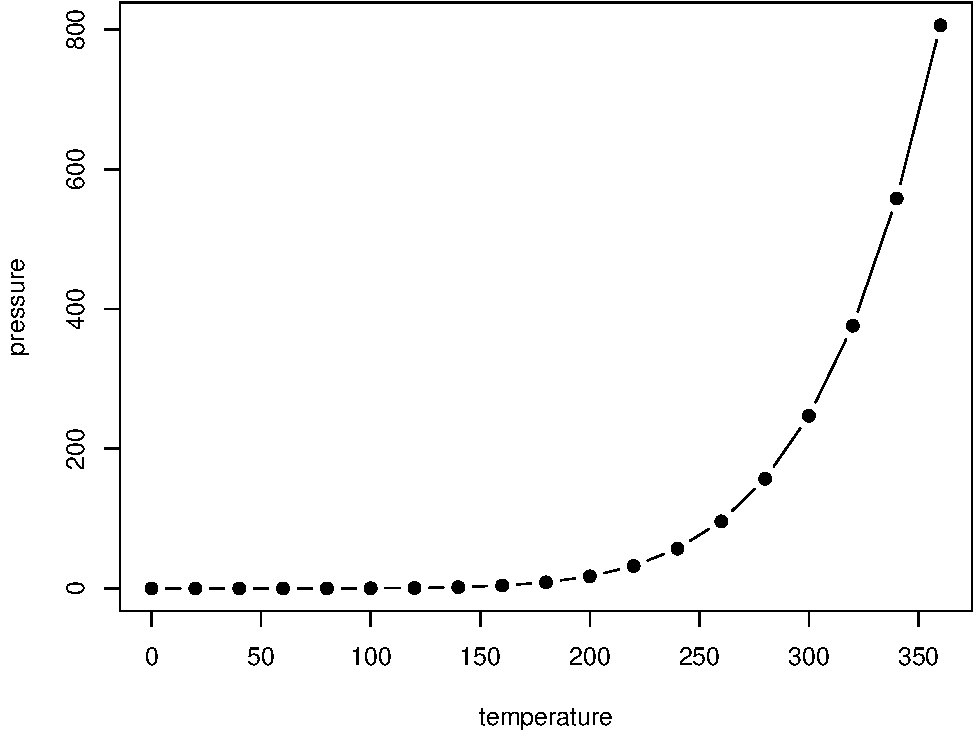
\includegraphics[width=0.8\linewidth]{book-MQ_files/figure-latex/nice-fig-1} 

}

\caption{Here is a nice figure!}\label{fig:nice-fig}
\end{figure}

Don't miss Table \ref{tab:nice-tab}.

\begin{table}

\caption{\label{tab:nice-tab}Here is a nice table!}
\centering
\begin{tabular}[t]{rr}
\toprule
temperature & pressure\\
\midrule
0 & 0.0002\\
20 & 0.0012\\
40 & 0.0060\\
60 & 0.0300\\
80 & 0.0900\\
\addlinespace
100 & 0.2700\\
120 & 0.7500\\
140 & 1.8500\\
160 & 4.2000\\
180 & 8.8000\\
\bottomrule
\end{tabular}
\end{table}

\hypertarget{dinamica-particulas}{%
\chapter{Dinâmica de partículas}\label{dinamica-particulas}}

All chapters start with a first-level heading followed by your chapter title, like the line above. There should be only one first-level heading (\texttt{\#}) per .Rmd file.

\hypertarget{a-section}{%
\section{A section}\label{a-section}}

All chapter sections start with a second-level (\texttt{\#\#}) or higher heading followed by your section title, like the sections above and below here. You can have as many as you want within a chapter.

\hypertarget{an-unnumbered-section}{%
\subsection*{An unnumbered section}\label{an-unnumbered-section}}
\addcontentsline{toc}{subsection}{An unnumbered section}

Chapters and sections are numbered by default. To un-number a heading, add a \texttt{\{.unnumbered\}} or the shorter \texttt{\{-\}} at the end of the heading, like in this section.

\hypertarget{parts}{%
\chapter{Parts}\label{parts}}

You can add parts to organize one or more book chapters together. Parts can be inserted at the top of an .Rmd file, before the first-level chapter heading in that same file.

Add a numbered part: \texttt{\#\ (PART)\ Act\ one\ \{-\}} (followed by \texttt{\#\ A\ chapter})

Add an unnumbered part: \texttt{\#\ (PART\textbackslash{}*)\ Act\ one\ \{-\}} (followed by \texttt{\#\ A\ chapter})

Add an appendix as a special kind of un-numbered part: \texttt{\#\ (APPENDIX)\ Other\ stuff\ \{-\}} (followed by \texttt{\#\ A\ chapter}). Chapters in an appendix are prepended with letters instead of numbers.

\hypertarget{teoria-ondulatoria}{%
\chapter{Teoria ondulatória}\label{teoria-ondulatoria}}

All chapters start with a first-level heading followed by your chapter title, like the line above. There should be only one first-level heading (\texttt{\#}) per .Rmd file.

\hypertarget{a-section-1}{%
\section{A section}\label{a-section-1}}

All chapter sections start with a second-level (\texttt{\#\#}) or higher heading followed by your section title, like the sections above and below here. You can have as many as you want within a chapter.

\hypertarget{an-unnumbered-section-1}{%
\subsection*{An unnumbered section}\label{an-unnumbered-section-1}}
\addcontentsline{toc}{subsection}{An unnumbered section}

Chapters and sections are numbered by default. To un-number a heading, add a \texttt{\{.unnumbered\}} or the shorter \texttt{\{-\}} at the end of the heading, like in this section.

\hypertarget{footnotes-and-citations}{%
\chapter{Footnotes and citations}\label{footnotes-and-citations}}

\hypertarget{footnotes}{%
\section{Footnotes}\label{footnotes}}

Footnotes are put inside the square brackets after a caret \texttt{\^{}{[}{]}}. Like this one \footnote{This is a footnote.}.

\hypertarget{citations}{%
\section{Citations}\label{citations}}

Reference items in your bibliography file(s) using \texttt{@key}.

For example, we are using the \textbf{bookdown} package (\protect\hyperlink{ref-R-bookdown}{Xie 2022}) (check out the last code chunk in index.Rmd to see how this citation key was added) in this sample book, which was built on top of R Markdown and \textbf{knitr} (\protect\hyperlink{ref-xie2015}{Xie 2015}) (this citation was added manually in an external file book.bib).
Note that the \texttt{.bib} files need to be listed in the index.Rmd with the YAML \texttt{bibliography} key.

The RStudio Visual Markdown Editor can also make it easier to insert citations: \url{https://rstudio.github.io/visual-markdown-editing/\#/citations}

\hypertarget{part-tuxf3picos-de-mecuxe2nica-quuxe2ntica}{%
\part{Tópicos de mecânica quântica}\label{part-tuxf3picos-de-mecuxe2nica-quuxe2ntica}}

\hypertarget{fundamentos-mq}{%
\chapter{Fundamentos da mecânica quântica}\label{fundamentos-mq}}

\hypertarget{blocks}{%
\chapter{Blocks}\label{blocks}}

\hypertarget{equations}{%
\section{Equations}\label{equations}}

Here is an equation.

\begin{equation} 
  f\left(k\right) = \binom{n}{k} p^k\left(1-p\right)^{n-k}
  \label{eq:binom}
\end{equation}

You may refer to using \texttt{\textbackslash{}@ref(eq:binom)}, like see Equation \eqref{eq:binom}.

\hypertarget{theorems-and-proofs}{%
\section{Theorems and proofs}\label{theorems-and-proofs}}

Labeled theorems can be referenced in text using \texttt{\textbackslash{}@ref(thm:tri)}, for example, check out this smart theorem \ref{thm:tri}.

\begin{theorem}
\protect\hypertarget{thm:tri}{}\label{thm:tri}For a right triangle, if \(c\) denotes the \emph{length} of the hypotenuse
and \(a\) and \(b\) denote the lengths of the \textbf{other} two sides, we have
\[a^2 + b^2 = c^2\]
\end{theorem}

Read more here \url{https://bookdown.org/yihui/bookdown/markdown-extensions-by-bookdown.html}.

\hypertarget{callout-blocks}{%
\section{Callout blocks}\label{callout-blocks}}

The R Markdown Cookbook provides more help on how to use custom blocks to design your own callouts: \url{https://bookdown.org/yihui/rmarkdown-cookbook/custom-blocks.html}

\hypertarget{sharing-your-book}{%
\chapter{Sharing your book}\label{sharing-your-book}}

\hypertarget{publishing}{%
\section{Publishing}\label{publishing}}

HTML books can be published online, see: \url{https://bookdown.org/yihui/bookdown/publishing.html}

\hypertarget{pages}{%
\section{404 pages}\label{pages}}

By default, users will be directed to a 404 page if they try to access a webpage that cannot be found. If you'd like to customize your 404 page instead of using the default, you may add either a \texttt{\_404.Rmd} or \texttt{\_404.md} file to your project root and use code and/or Markdown syntax.

\hypertarget{metadata-for-sharing}{%
\section{Metadata for sharing}\label{metadata-for-sharing}}

Bookdown HTML books will provide HTML metadata for social sharing on platforms like Twitter, Facebook, and LinkedIn, using information you provide in the \texttt{index.Rmd} YAML. To setup, set the \texttt{url} for your book and the path to your \texttt{cover-image} file. Your book's \texttt{title} and \texttt{description} are also used.

This \texttt{gitbook} uses the same social sharing data across all chapters in your book- all links shared will look the same.

Specify your book's source repository on GitHub using the \texttt{edit} key under the configuration options in the \texttt{\_output.yml} file, which allows users to suggest an edit by linking to a chapter's source file.

Read more about the features of this output format here:

\url{https://pkgs.rstudio.com/bookdown/reference/gitbook.html}

Or use:

\hypertarget{refs}{}
\begin{CSLReferences}{1}{0}
\leavevmode\vadjust pre{\hypertarget{ref-xie2015}{}}%
Xie, Yihui. 2015. \emph{Dynamic Documents with {R} and Knitr}. 2nd ed. Boca Raton, Florida: Chapman; Hall/CRC. \url{http://yihui.org/knitr/}.

\leavevmode\vadjust pre{\hypertarget{ref-R-bookdown}{}}%
---------. 2022. \emph{Bookdown: Authoring Books and Technical Documents with r Markdown}. \url{https://CRAN.R-project.org/package=bookdown}.

\end{CSLReferences}

\end{document}
